\documentclass[12pt,answers]{exam}


\usepackage{cmap, type1ec}
\usepackage[T2A]{fontenc}
\usepackage[utf8]{inputenc}
\usepackage[russian]{babel}

\usepackage{xcolor}
\usepackage{hyperref}
\usepackage{alltt}

\hypersetup{%
  colorlinks=false,% hyperlinks will be black
  linkbordercolor=blue,% hyperlink borders will be red
  pdfborderstyle={/S/U/W 1}% border style will be underline of width 1pt
}

\usepackage[margin=1in]{geometry}
\usepackage{amsmath,amssymb}
\usepackage{multicol}
\usepackage{etoolbox}

\usepackage{float}
\usepackage{siunitx}

\usepackage{tikz}
\usetikzlibrary{trees}
\usetikzlibrary{shapes.geometric}
\usetikzlibrary{positioning}

\newcommand{\class}{Теория алгоритмов}
\newcommand{\term}{Весенний семестр 2017}
\newcommand{\examnum}{Письменный экзамен}
\newcommand{\examdate}{26 июня 2017}
\newcommand{\timelimit}{16:40 -- 18:40}

\pagestyle{head}
\firstpageheader{}{}{}
\runningheader{\class}{\examnum\ - Страница \thepage\ из \numpages}{\examdate}
\runningheadrule

\providecommand{\abs}[1]{\left\lvert{#1}\right\rvert}

\renewcommand{\solutiontitle}{}

\makeatletter
\newcommand{\iftoggleverb}[1]{%
  \ifcsdef{etb@tgl@#1}
    {\csname etb@tgl@#1\endcsname\iftrue\iffalse}
    {\etb@noglobal\etb@err@notoggle{#1}\iffalse}%
}
\makeatother

\graphicspath{{./figures/}}

\begin{document}

\noindent
\begin{tabular*}{\textwidth}{l @{\extracolsep{\fill}} r @{\extracolsep{6pt}} l}
\textbf{\class} & \textbf{Студент:} & \makebox[3in]{\hrulefill}\\
\textbf{\term} &&\\
\textbf{\examnum} &&\\
\textbf{\examdate} \\
\textbf{\timelimit}
\end{tabular*}\\
\rule[2ex]{\textwidth}{2pt}%
\begin{center}
Оценки (заполняется преверяющими)\\
\addpoints
\gradetable[h][questions]
\end{center}
\noindent
\rule[2ex]{\textwidth}{2pt}

\begin{questions}


\question[5] Отметьте, является ли утверждение истинным. Обосновывать свой выбор не требуется.
\begin{parts}
  %\choice
  \part {\em Степенью захода} вершины направленного графа $G=(V, E)$ называется число рёбер {\em входящих} в вершину. Имея представление $G$ в виде списка смежных вершин, степени захода всех вершин можно вычислить за $O(V)$.
  \begin{solution}
    Неверно. В данном представлении граф является словарём, где каждый ключ обозначает некоторую вершину графа $v$, а его значение – список вершин, в которые из $v$ имеются рёбра.

    Чтобы найти {\em степень захода} вершин, потребуется посчитать, сколько раз каждая из них встречается в вышеупомянутых списках. Для этого их надо обойти целиком. Суммарно во всех списках $\abs{E}$ элементов, исследовать списки надо в каждом из $\abs{V}$ ключей. Итоговая сложность – $O(V+E)$
  \end{solution}

  %\CorrectChoice
  \part Поиск в ширину в ненаправленном графе без весов позволяет найти кратчайшие пути от некоторой вершины $s$ до всех остальных вершин.
  \begin{solution}
    Верно. Доказательство, например, в CLRS 22.2
  \end{solution}

  %\CorrectChoice
  \part Рассмотрим взвешеный направленный граф $G=(V,E,w)$ с кратчайшим путём $p$ между вершинами $s$ и $t$. В графе $G'=(V,E,w')$, где вес каждого ребра из $G$ был удвоен, $p$ по-прежнему является кратчайшим путём.
  \begin{solution}
    Верно. Любой путь – линейная комбинация весов $\sum w_i$. При удвоении весов удвоятся и все длины всех путей между $s$ и $t$, что не повлияет на их относительный порядок.
  \end{solution}

  % \choice
  \part Рассмотрим направленный граф $G=(V,E,w)$ содержащий циклы с отрицательной суммой. Алгоритм Беллмана-Форда позволяет найти в $G$ кратчайшие ациклические пути от некоторой начальной вершины $s$ до остальных вершин.
  \begin{solution}
    Неверно. Алгоритм Беллмана-Форда лишь сигнализирует о том, что в графе есть циклы с отрицательной суммой.
  \end{solution}

  %\choice
  \part Для каждого связного ненаправленного графа существует ровно одно минимальное покрывающее дерево.
  \begin{solution}
    Неверно. В графе с рёбрами одинакового веса может быть \href{https://upload.wikimedia.org/wikipedia/commons/c/c9/Multiple_minimum_spanning_trees.svg}{несколько MST}.
  \end{solution}
\end{parts}

\question
Дан отсортированный массив целых чисел.
\begin{parts}

\part[2] Опишите (подробным текстом или псевдокодом) рекурсивный алгоритм построения {\em сбалансированного} бинарного дерева поиска из этого массива.

{\em Указание:} здесь не требуется использовать специальные структуры данных вроде красно-чёрных деревьев.
  \begin{solution}
    Делаем медиану (в отсортированном массиве – средний элемент) корнем, дерева, левую и правую части массива отсылаем в соответствующие поддеревья. Рекурсивно проделываем то же самое для поддеревьев.
  \end{solution}

\part[2]
Найдите асимптотическое время работы алгоритма.

{\em Указание:} в этом вам может помочь master theorem.
  \begin{solution}
    Время работы такого алгоритма записывается рекурсивно:
    $$
      T(n) = 2 T(n/2) + O(1)
    $$
    То есть соответствует рекуррентности из master theorem:
    $$
      T(n) = aT(n/b) + f(n)
    $$
    при $a=2$, $b=2$, $f(n)=1$. Из трёх возможных в master theorem оценок нам подходит $f(n) = O(n^{\log_b a - \epsilon}) = O(n^{1 - \epsilon})$ где $\epsilon=1$. Следовательно, $T(n) = \Theta(n^{\log_b a}) = \Theta(n)$
  \end{solution}
\end{parts}

\question[3]
Напишите рекурсивную функцию, которая принимает два бинарных дерева и возвращает {\tt True} если они равны (т.е. имеют одинаковую структуру и значения в узлах).

\begin{solution}
  \begin{alltt}
    def is_same_tree(p, q):
        
        if p and q:
            return (
              p.val == q.val
              and is_same_tree(p.left, q.left)
              and is_same_tree(p.right, q.right)
            )
        
        # Are both elements None?
        return p is q
  \end{alltt}
\end{solution}

\question[3]
Дано множество $S$ из $n$ точек на плоскости. Стоит задача найти кратчайший (в смысле эвклидового расстояния на плоскости) циклический путь, проходящий через все точки. Не вдаваясь в необходимые структуры данных, придумайте и опишите некоторый {\em жадный} алгоритм для приближённого решения такой задачи. Приведите два примера $S$, когда ваш алгоритм приведёт к оптимальному и неоптимальному решениям.

\begin{solution}
Возможное решение: последовательно добавлять в путь точки, являющиеся ближайшими к 
последним добавленным. Решение будет оптимальным, например, для точек, равномерно распределённых на окружности. Пример неоптимального решения:
\begin{figure}[H]
  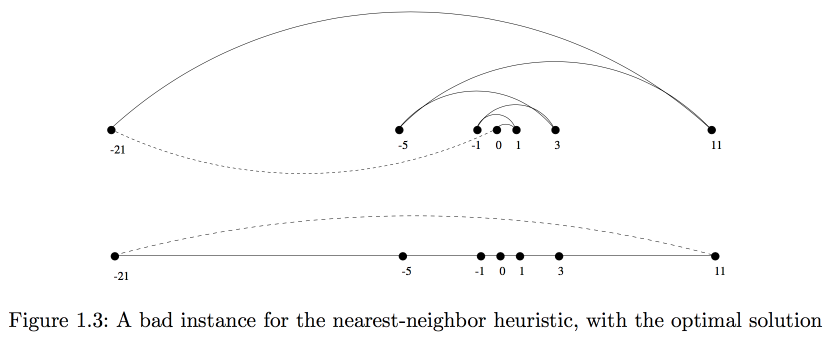
\includegraphics[width=15cm]{points.png}
\end{figure}
\end{solution}


\question[6]
Вычислять биномиальные коэффициенты $\binom{n}{k}$ по прямой формуле
$$
\binom{n}{k} = \frac{n!}{(n-k)!~k!}
$$
неудобно из-за необходимости производить арифметические операции над очень большими числами в промежуточных вычислениях. Например, $100! \approx \num{9.3e157}$, при этом $\binom{100}{90}\approx \num{1.73e13}$
Используя динамическое программирование и соотношение
$$
\binom{n}{k} = \binom{n-1}{k-1} + \binom{n-1}{k}
$$
опишите алгоритм, который лишён этого недостатка.

\begin{solution}
Заводим пустой двумерный массив {\tt D[][]}. Проверяем, есть ли там значение {\tt D[n][k]}. Если есть, возвращаем его. Если нет, применяем разложение в сумму, и рекурсивно вычисляем новые биномиальные коэффициенты и складываем. Результат записываем в массив {\tt D}.

Разложение следует продолжать пока не встретим базовые случаи: $\binom{i}{0} = 1$ и $\binom{i}{i} = 1$.

Подробнее смотрите, например, Skiena 8.1.4
\end{solution}


\question[3]
\begin{alltt}
$ man tsort 

NAME
     tsort -- topological sort of a directed graph

DESCRIPTION
     tsort takes a list of pairs of node names representing directed arcs
     in a graph and prints the nodes in topological order on standard output.

<...>

$ tsort <<EOF
> 3 8
> 3 10
> 5 11
> 7 8
> 7 11
> 8 9
> 11 2
> 11 9
> 11 10
> EOF
\end{alltt}

Что напечатает (а точнее, что {\em может} напечатать) программа?

  \begin{solution}
    Один из возможных вариантов топологической сортировки:
    $$
    7~~5~~3~~11~~10~~8~~2~~9
    $$
    Проверить это можно, нарисовав рёбра прямо на этой последовательности. Ни одно из рёбер не будет идти справа налево.
  \end{solution}

\newpage

\question[5]
Дан связный ненаправленный взвешенный граф $G=(V,E,w)$, причём все веса на его рёбрах различны. В $G$ присутствует цикл $\langle v_1, v_2, ... v_k, v_{k+1} \rangle$, где $v_{k+1} = v_1$. Пусть среди всех ребёр в этом цикле $\langle v_i, v_{i+1} \rangle$ имеет наибольший вес. Докажите что $\langle v_i, v_{i+1} \rangle$ не будет принадлежать ни одному минимальному покрывающему дереву (minimum spanning tree) в $G$.

  \begin{solution}
    Пусть существует MST, в который входит ребро $\langle v_i, v_{i+1} \rangle$. Удалив его из MST, возникает три варианта:
    \begin{itemize}
      \item Дерево по-прежнему содержит все вершины $G$. Значит, дерево изначально не являлось MST.
      \item Дерево перестало содержать вершину $v_i$. Тогда мы добавляем в MST ребро $\langle v_{i-1}, v_{i} \rangle$, вес которого меньше, чем у удалённого. Значит, дерево изначально не являлось MST.
      \item Аналогично рассуждаем если от дерева отрывается $v_{i+1}$
    \end{itemize}

    Приходим к противоречию: MST не может содержать $\langle v_i, v_{i+1} \rangle$.
  \end{solution}

\question[7]
Направленный граф $G=(V,E,w)$ на рисунке ниже представляет собой дорожную сеть. Вершины $V$ обозначают города, а рёбра $E$ -- платные дороги между ними. Вес $w(e)$ обозначает стоимость проезда по дороге $e$, а $w(v)$ обозначает стоимость заправки в городе $v$. Стоимость заправки фиксирована и не зависит от количества оставшегося бензина, при этом бак всегда заправляется полностью. Если $w(v)=\infty$, заправки в этом городе нет. На полном баке бензина можно пересечь {\em не более двух дорог.}

Ваша цель: {\em найти самый дешёвый маршрут из города $s$ в город $t$}. Перед самым началом пути в машину уже заправлен полный бак.

Казалось бы, дешевле всего ехать маршрутом
$\langle s, u_1, u_2, t \rangle$, всего за \$8.
К сожалению, этот маршрут не подходит, потому что по прибытию в $u_2$ у нас кончится бензин, и мы не сможем заправиться.
Зато точно подходит маршрут
$\langle s, u_3, u_2, t \rangle$ стоимостью \$22. Но он, очевидно, не самый дешёвый.

Опишите преобразование графа, которое сведёт исходную задачу к классической задаче поиска кратчайшего пути (где минимизируется сумма весов на рёбрах вдоль пути, и которую мы уже умеем искать с помощью алгоритма Дейкстры).

\begin{solution}
Полное решение смотрите по \href{https://ocw.mit.edu/courses/electrical-engineering-and-computer-science/6-006-introduction-to-algorithms-fall-2011/exams/MIT6_006F11_quiz2_sol.pdf}{ссылке}, Problem 6.

Его идея в том, чтобы выразить дополнительные переменные состояния автомобиля (количество бензина и платную заправку) в структуре графа.

В каждом городе автомобиль может быть заправлен полностью ($F$), наполовину ($H$), или с пустым баком ($E$). Соответственно, каждую вершину исходного графа надо поделить на три, обозначив их упомянутыми буквами.

Далее, если между городами есть ребро, следуем добавить рёбра с той же стоимостью между ($F$) и ($H$) одного города к, соответственно, ($H$) и ($E$) другого. Заправка бака в городе обозначается ребрами $(H, F)$ и $(E, F)$ в пределах одного города.

Поиск кратчайшего пути в таком графе даст самый дешёвый марштур, если он существует.
\end{solution}

\nomorequestions

\begin{figure}[!ht]
  \label{fig:roads}
  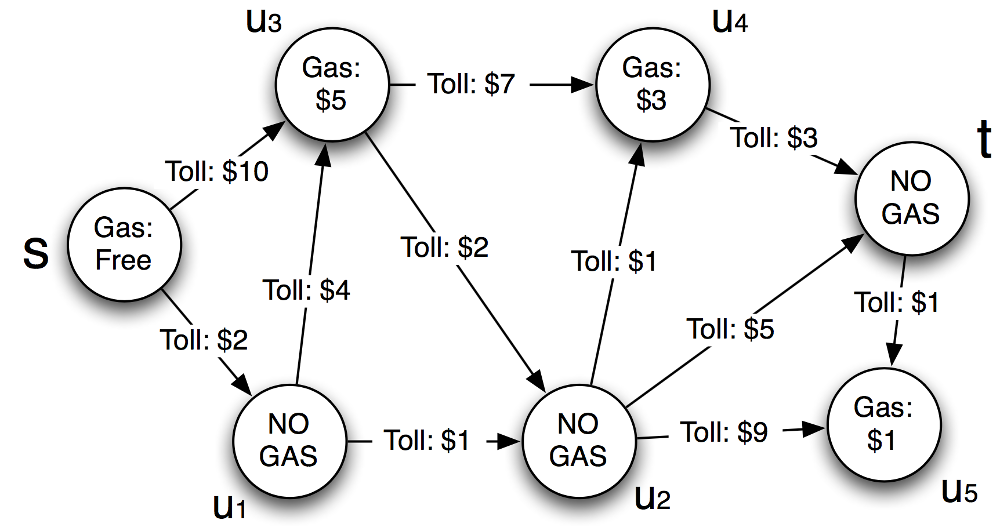
\includegraphics[width=15cm]{roads.png}
  \caption{Граф платных дорог и заправок.}
\end{figure}

\end{questions}

\end{document}
